\chapter{Návrh}\label{chap:design}

V této kapitole se bude zabývat návrhem úprav a rozšíření původní testovací knihovny


\section{Souhrn požadavků}

K tomu abych mohl správně navrhnout úpravy v testovací knihovně, tak je dobré připomenout, co se od nové knihovny požaduje a proč. Knihovna by ve své nové podobě měla umět spouštět virtualizovaná zařízení a dle konfigurace vytvářet požadované topologie. Hlavní motivací je zvýšení flexibility knihovny, rozšíření možností využití a minimalizovaní zásahu do kódu testovaného zařízení, což vše vede ke snížení nákladů a úsilí na testování.  

Tyto kroky směřují k snížení závislosti na reálném hardwaru, na kterém daný produkt následně poběží. Hardware a primárně jeho architektura ve spoustě případů hraje důležitou roli. Jsou ovšem komponenty, jejichž chování je stejné, ať už poběží na jakémkoliv stroji. Jejich logika si nijak nemění. Přesunutím testů těchto komponent do virtualizovaného prostředí rozšíří možnosti, jak tyto komponenty testovat. Zároveň je možné mít mnohem více testovacích scénářů na různých topologiích. Je ale samozřejmé, že testy na reálném hardwaru budou vždy potřeba a nelze se této závislosti nijak zbavit.


\section{Návrh změny architektury}

Jednu z možných architektur stávající testovací knihovny bylo možné vidět na obrázku \ref{fig:bp_devicemodel}. Předchozí přístup vyžadoval existenci alespoň jednoho fyzického zařízení, tedy reálného zařízení běžícího mimo zařízení, na kterém byla spouštěna testovací knihovna. Toto byla velice omezující podmínka, díky které nebylo možné virtualizovat samotné testované zařízení.

Představu nové architektury je možné vidět na obrázku \ref{fig:architecture}. Jak je na obrázku vidět, vše se již odehrává na tzv. agentovi, což je ve finále jakékoliv zařízení s potřebným softwarem pro virtualizaci. Všechna zařízení, mimo testovací služby, jsou přesunuta do virtualizovaného prostředí, které bude orchestrováno za pomoci softwaru Docker. 

\begin{figure}[htbp]
    \centering 
    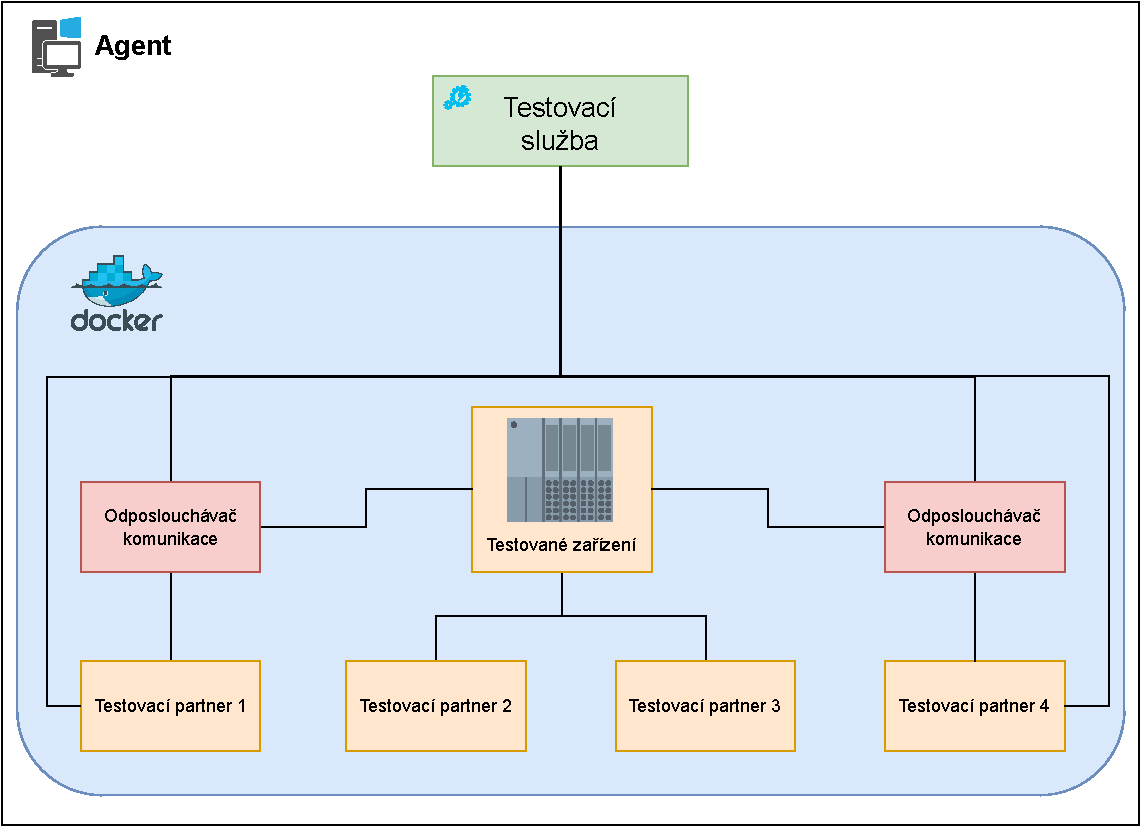
\includegraphics[width=\textwidth]{assets/img/architecture.pdf}
    \caption{Ukázka jedné z možných architektur nové testovací knihovny}
    \label{fig:architecture}
\end{figure}

Na obrázku lze vidět tři druhy zařízení, která jsou barevně oddělená. Zeleně označeným zařízením je původní \textit{testovací služba}. Ta řídí testovací běh a vyhodnocuje výsledky testů. Testovací služba běží přímo v operačním systému agenta, tedy bez žádné virtualizace. 

Uvnitř modře označeného nového virtualizovaného prostředí lze následně vidět jednu z možných simulovaných topologií, v tomto případě topologii hvězdy. Každý objekt uvnitř virtualizovaného prostředí představuje právě jedno zařízení, které je kontejnerizováno. Všechna oranžově označená virtualizovaná zařízení představují účastníky testu, tedy zařízení, které nějak přispívají k provedení daného testu. \textit{Testované zařízení} představuje vyvíjený produkt, který chceme testovat. Ostatní oranžová zařízení představují \textit{testovací partnery}. Ti přispívají k vytvoření prostředí testu a k orchestraci testu.

Rozdílem od stávající knihovny je, že ne všichni účastníci testu musí být k testovací službě připojeni. Na obrázku lze vidět, že v tomto případě pouze testovací partner 1 a 4 jsou připojeni k testovací službě. Je zde ale předpoklad, že alespoň jedno zařízení musí být k testovací službě připojeno.

Novým typem zařízení je červeně označený \textit{odposlouchávač komunikace}. Toto zařízení, jak už z názvu vyplývá, bude zaznamenávat komunikaci na právě jednom spojení dvou zařízení. Zároveň bude připojeno k testovací službě. Díky tomuto spojení bude možné zaznamenávat komunikaci pouze v průběhu testu, což ve výsledku bude znamenat, že pro každý test bude existovat separátní záznam komunikace.


\subsection{Propojení s externími komponentami}

Testovací knihovna bude využívat k testování tyto komponenty:

\begin{itemize}
    \item Testovací knihovnu MSTest
    \item Kontejnerizační řešení Docker
\end{itemize}

Každá komponenta má své důležité využití. Testovací knihovna MSTest, která je již využita ve stávající knihovně, umožňuje testy spouštět, díky její široké integraci. Díky ní je mimo jiné možné testy spouštět na Azure DevOps, za pomocí než lze dosáhnout plné automatizace testování.

S pomocí virtualizačního řešení Docker bude knihovna následně schopna vytvářet jednotlivá virtualizovaná zařízení a následně je propojovat mezi sebou do požadovaných topologií. 

To vše umožní testovací knihovně úspěšně testovat. Jejich propojení můžeme vidět na obrázku \ref{fig:run_stack}. Jak lze vidět, testovací knihovna je ovládána prostřednictvím testovací knihovny MSTest. Ta poté provede všechny potřebné operace, jako vytvoření testovací služby a vytvoření virtualizovaného prostředí, které je vytvářeno pomocí softwaru Docker. Všechny vytvořené zdroje jsou poté na konci testování odstraněny.  

\begin{figure}[htbp]
    \centering 
    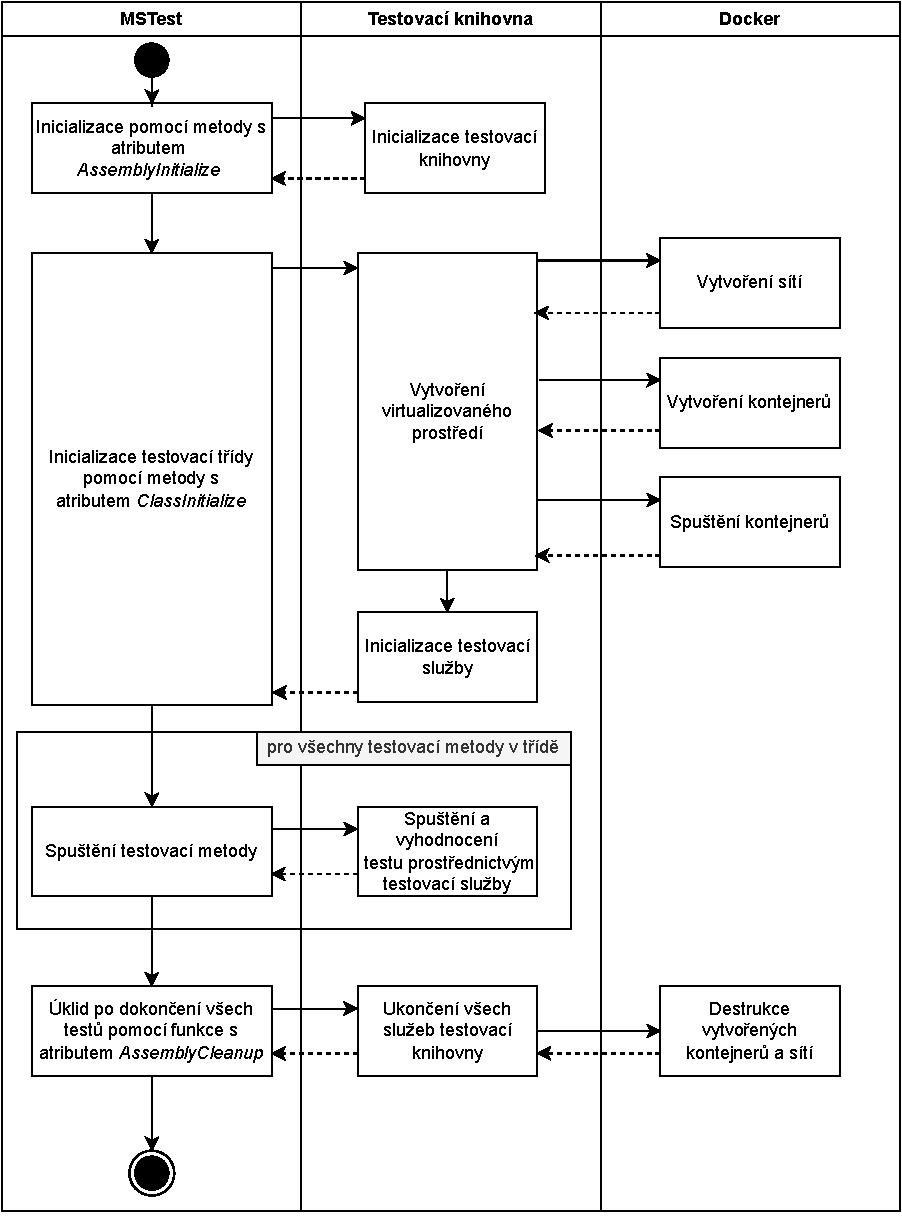
\includegraphics[width=\textwidth]{assets/img/run_stack.pdf}
    \caption{Propojení a komunikace mezi komponenty v testovací knihovně}
    \label{fig:run_stack}
\end{figure}


\section{Orchestrace virtualizovaného prostředí}

Důležitou součástí testovací knihovny bude implementace orchestrace virtualizovaného prostředí. To znamená, že testovací služba bude schopna vytvářet jednotlivá virtuální zařízení, které následně automaticky propojí dle požadované topologie a po konci testování daná zařízení ukončí. 

Knihovna bude obsahovat tzv. \textit{správce virtualizovaného prostředí}. Ten se bude starat o všechny úkony spojené s vytvářením a chodem virtualizovaného prostředí. Tedy tento správce bude vytvářet potřebné kontejnery a sítě, s pomocí niž propojí všechna zařízení dle konfigurace. 

\subsection{Nastavení virtualizovaného prostředí}\label{sec:env_conf}

Virtualizované prostředí bude definované za pomoci konfiguračního souboru dle formátu YAML. Hlavní důvod proč využít YAML, místo původního formátu JSON, kterým bylo definováno nastavení testovací knihovny, je co nejbližší přiblížení se aktuálním konvencím v kontextu k Docker compose. Konfigurace bude tedy co nejvíce napodobovat jeho konfigurační soubor. 

První položkou v konfiguračním souboru bude položka \inlinecode{label}. Ta bude obsahovat označení daného virtualizovaného prostředí. Další položkou v konfiguračním souboru bude položka \inlinecode{service}. Ta bude obsahovat pouze položku \inlinecode{connections}, která bude obsahovat počet zařízení, která se připojí k testovací službě. Toto číslo musí být větší než 0.

Další položkou bude položka \inlinecode{containers}. Ta bude obsahovat informace o všech zařízeních, která v daném virtualizovaném prostředí budou. Klíčem každé položky uvnitř této sekce bude název zařízení, které bude fungovat pro referenci daného zařízení. Pro každé zařízení následně půjde definovat tato nastavení: 

\begin{description}
    \item[build] Definice zařízení, buď za pomoci obrazu (image) nebo cestou k docker souboru (Dockerfile). Toto bude označeno klíčem \inlinecode{image} a \inlinecode{dockerfile}, následovanou požadovanou hodnotou.
    \item[cap\_add] Seznam \uv{schopností}, v tomto kontextu práv, které bude daný účet na kontejneru mít. Ty budou přidány ke právům, které v základu docker dává účtu vytvořenému v kontejneru. 
    \item[commands] Seznam příkazů, které budou spuštěny v kontejneru.
    \item[environment] Seznam proměnných, která budou v kontejneru nastaveny. Klíč bude název proměnné a jeho hodnota bude hodnotou proměnné
    \item[ip\_mapping] Seznam mapování IP adres na domény. Klíčem je název domény a hodnotou je IP adresa, na kterou má daná doména ukazovat.
    \item[ports] Seznam mapování portů z kontejneru do prostředí hostitelského zařízení. Každý záznam obsahuje dva porty oddělené dvojtečkou, kdy první je port hostitelského zařízení a druhý je port kontejnerizovaného zařízení.
    \item[privileged] Boolean hodnota, která při hodnotě \inlinecode{true} přiřadí účtu správcovská práva
    \item[logging] Boolean hodnota, která značí zdali je komunikace mezi tímto zařízením odposlouchávána. Tedy pokud je hodnota \inlinecode{true}, tak poté knihovna zařídí zaznamenávání všech spojů tohoto zařízení
    \item[type] Typ zařízení, které bude vytvořeno. Typy zařízení jsou blíže vysvětleny v sekci \ref{sec:cont_design}.
    \item[tty] Boolean hodnota, která v původním docker compose značí připojení pseudo-terminálu ke kontejneru, který má za následek to, že kontejner po dokončení definovaných příkazů zůstane běžet. V kontextu knihovny bude znamenat to, že kontejner zůstane po dokončení všech příkazů definovaných v \inlinecode{commands} běžet. 
\end{description}

V neposlední řadě konfigurační soubor bude obsahovat položku \inlinecode{links}. Ta bude definovat jednotlivá propojení mezi zařízeními, tedy celkovou topologii. V tomto seznamu bude každá položka obsahovat názvy dvou zařízení oddělené dvojtečkou a pro každý záznam bude vytvořeno propojení mezi danými zařízeními.

Povinnou součástí konfiguračního souboru bude celá sekce \inlinecode{service}, sekce \inlinecode{containers}, kde musí být definována nejméně jedno zařízení, která musí obsahovat alespoň kolonky \inlinecode{build} a \inlinecode{type}. Ostatní budou nepovinné. Platí zde ale podmínka, že každé zařízení musí dosáhnout všech ostatních zařízení ve virtualizovaném prostředí.

Testovací knihovna bude kontrolovat, zdali testované prostředí bylo vytvořeno. Pokud ne, nezapočne testování. Zároveň bude kontrolovat zda všechna zařízení byla úspěšně spuštěna. Po konci testování testovací knihovna všechna zařízení ukončí, a vymaže všechny jím definované sítě, kontejnery atd.

Pro pohodlnost testovací knihovna bude také podporovat více různých topologií v rámci jednoho testovacího projektu. Při každé inicializaci virtualizovaného prostředí testovací služba porovná danou konfiguraci s aktuální konfigurací. Pokud budou konfigurace totožné, testovací služba ponechává prostředí nepozměněné, v opačném případě vyčistí virtualizované prostor, do kterého následně vloží nová zařízení a jejich nastavení. 

\subsection{Definice zařízení}\label{sec:cont_design}

Testovací knihovna bude pro definici kontejnerizovaného zařízení obsahovat rozhraní pod názvem \inlinecode{IVMContainer}. Toto rozhraní bude obsahovat následující metody:

\begin{itemize}
    \item \inlinecode{SetNetworkConf(ContainerNetworkConf)} - přidá nastavení sítě.
    \item \inlinecode{AddCommand(string)} - přidá příkaz, který bude spuštěn po spuštění kontejneru.
    \item \inlinecode{SetEnvironmentVariables(Dictionary<string, string>)} - přidá proměnné do prostředí kontejneru.
    \item \inlinecode{AddCapability(string)} - přidá schopnost, neboli práva, kontejneru.
    \item \inlinecode{RunPriviledged()} - dá správcovská práva kontejneru.
    \item \inlinecode{ExposePort(int,int)} - zpřístupní port kontejneru do hostitelského zařízení. První argument je číslo portu v kontejneru, druhý argument je port, ze kterého daný port bude přístupný na hostitelském zařízení. 
    \item \inlinecode{Mount(string,string)} - zpřístupní složku na hostitelském zařízení v kontejneru. První argument je cesta na hostitelském zařízení, druhý cesta v kontejneru.
    \item \inlinecode{Tty()} - donutí kontejner běžet i po dokončení všech příkazů.
    \item \inlinecode{Build()} - sestaví daný kontejner.
    \item \inlinecode{Start()} - spustí daný kontejner. Metoda vrací boolean hodnotu o správnosti spuštění kontejneru.
    \item \inlinecode{Stop()} - zastaví daný kontejner.
    \item \inlinecode{Dispose()} - zničí všechny alokované prostředky, včetně vytvořeného kontejneru v Docker.
    \item \inlinecode{GetLog()} - získá z kontejneru všechny zápisy, které byly v něm vypsány
    \item \inlinecode{IsRunning} - vlastnost, která značí, zda daný kontejner je spuštěn
\end{itemize}

Správce virtualizovaného prostředí následně bude schopen nastavit daná zařízení dle implementace předem definovaného rozhraní. Druh implementace bude určen položkou \inlinecode{type} v konfiguraci zařízení. Každá implementace daného rozhraní musí zajistit správné nastavení všech konfiguračních položek definovaných rozhraním kontejnerizovaného zařízení.

\section{Komunikace}

Komunikaci v rámci testovací knihovny lze rozdělit do dvou kategorií:

\begin{enumerate}
    \item komunikace mezi zařízeními,
    \item komunikace s testovací službou.
\end{enumerate}

Veškerá komunikace mezi zařízeními bude probíhat uvnitř virtualizovaného prostředí. Jejich propojení bude zajištěno pomocí testovací knihovny. Ta dle konfigurace, definované v sekci \ref{sec:env_conf}, vytvoří jednotlivá propojení mezi zařízeními s pomocí softwaru Docker. Tato komunikace nebude nijak ze strany testovací knihovny kontrolována, pouze může být v průběhu testu zaznamenána. 

Testovací knihovna pro každé zařízení nastaví seznam interních domén, skrz které bude možné adresovat účastníky testu. Tyto domény budou ve tvaru \inlinecode{[jméno-zařízení].internal}. Validními znaky pro domény budou pouze písmena, čísla a pomlčka. Jméno zařízení tedy bude transformováno tak, aby obsahovalo pouze tyto znaky. Všechny nepodporované znaky budou z jména zařízení odstraněny. Výjimkou je pouze znak \inlinecode{'\_'}, který bude nahrazen pomlčkou. V případě kolize dvou jmen po transformaci bude do jména domény přidán index. 

Ukázku přiřazení domén můžeme vidět na obrázku \ref{fig:domain_resolving}. Jak je vidět, topologie je totožná s ukázkovou topologií na obrázku \ref{fig:architecture}, pouze ke všem zařízením uvnitř virtuálního prostředí bylo přiřazeno unikátní jméno. Každé zařízení má přiřazenou doménu dle daného formátu. Výjimkou je pouze testovací služba, která je mimo virtualizované prostředí. Software Docker automaticky definuje doménu \inlinecode{host.docker.internal}, s pomocí které je možné adresovat hostující stroj a tím pádem i testovací službu.

\begin{figure}[htbp]
    \centering 
    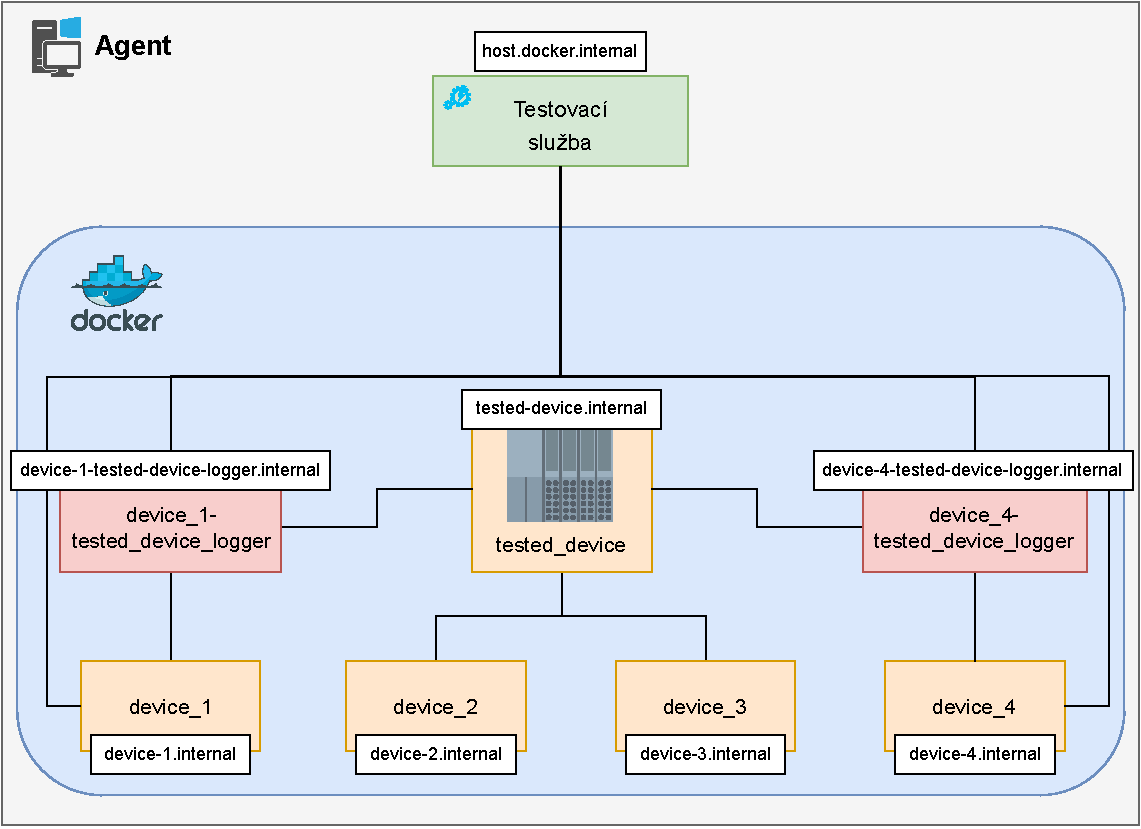
\includegraphics[width=\textwidth]{assets/img/domain_resolving.pdf}
    \caption{Ukázka přiřazení domén k zařízením}
    \label{fig:domain_resolving}
\end{figure}


Komunikace s testovací službou bude probíhat za stejných podmínek, jako tomu je doposud. Testovací knihovna přesně definuje strukturu zpráv. Každá zpráva obsahuje v prvních dvou bajtech typ zprávy, v dalších dvou bajtech délku dat zprávy a případná data zprávy, jejichž délka je uložena v délce dat zprávy. Každá zpráva tedy musí mít minimálně 4 bajty. Veškerá data zprávy jsou uloženy dle formátu \textit{big-endian}, respektive na paměťovém místě s nejnižší adresou je uložen nejvýznamnější bit.

Možnou komunikaci mezi testovací službou a účastníky testu, tedy zařízeními uvnitř virtualizovaného prostředí, můžeme vidět na sekvenčním diagramu, který je na obrázku \ref{fig:seqdiag}. Na něm lze vidět, jak by probíhala komunikace při běhu o jednom testu. Jak jsem již ale zmínil dříve, dle nového přístupu nemusí všechna zařízení komunikovat s testovací službou. 

\begin{figure}[htbp]
    \centering 
    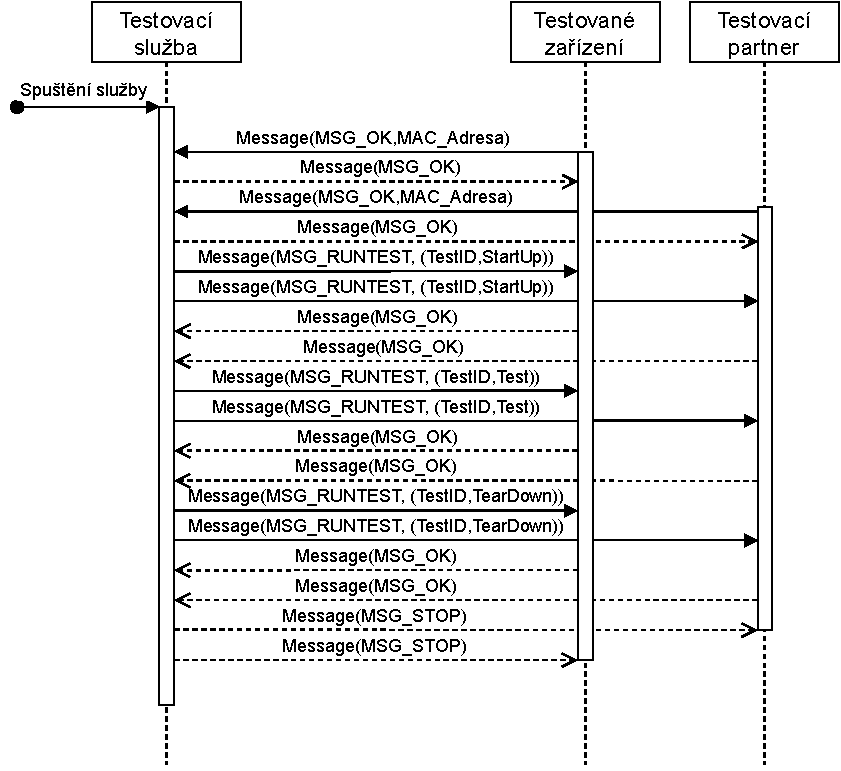
\includegraphics[width=\textwidth]{assets/img/bp_assets/sequencediagram.pdf}
    \caption{Sekvenční diagram ukázky komunikace mezi účastníky testování}
    \source{Převzato z \cite{bakalarka}}
    \label{fig:seqdiag}
\end{figure}

\section{Testovací služba}

Jádrem testovacího běhu zůstane testovací služba, která musí komunikovat a tím ovládat alespoň jedno zařízení. Ve stávající implementaci byla na počátku testování vytvořena jedna instance testovací služby, která existovala po celou dobu testování. Nově bude životnost testovací služba navázána na dané virtualizované prostředí. Tedy, testovací služba vznikne až po úspěšném vytvoření virtualizovaného prostředí. Při změně virtualizovaného prostředí bude testovací služba ukončena a po vytvoření nového prostředí spuštěna nová instance.

Fungování testovací služby lze vidět na novém diagramu aktivit testovací služby na obrázku \ref{fig:activitydiagramservice}, na kterém jsou označeny i změny oproti původnímu diagramu aktivit testovací služby. Jak lze z diagramu vidět, nově již nelze přidávat nové testovací partnery po dokončení inicializační fáze testovací služby.

\begin{figure}[htbp]
    \centering 
    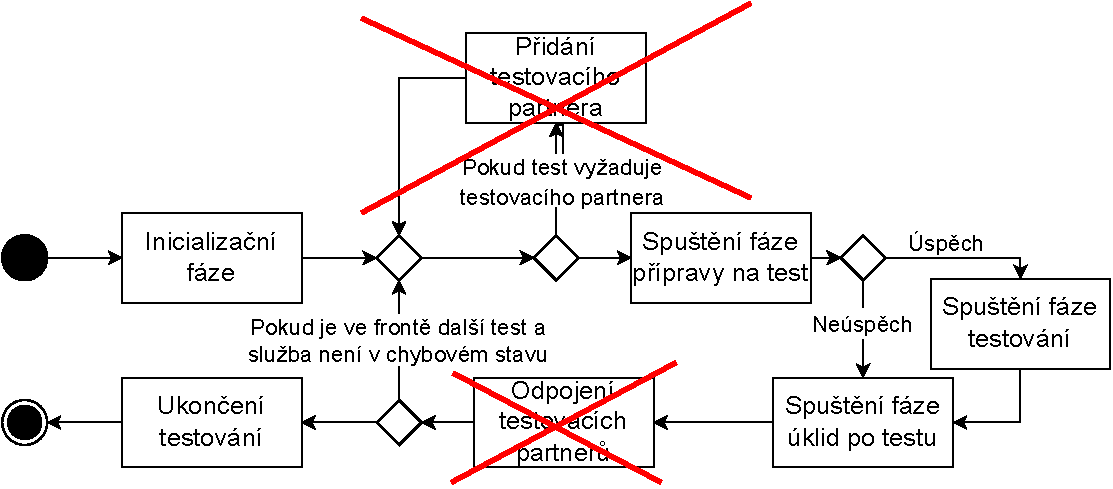
\includegraphics[width=\textwidth]{assets/img/activitydiagramservicechange.pdf}
    \caption{Nový diagram aktivit testovací služby}
    \source{Vytvořeno dle předlohy z \cite{bakalarka}}
    \label{fig:activitydiagramservice}
\end{figure}

Po sestavení virtualizovaného prostředí testovací služba započne inicializační fázi, ve které se všechna zařízení ovládaná testovací službou připojí k testovací službě. Tedy mimo přímých účastníků testu se v této fázi připojí i všichni odposlouchávači komunikace, pokud nějací existují. 

Testovací služba sama o sobě nemá ponětí o tom, které testy budou spuštěny a které ne. Testovací služba skrz definované API definuje metodu, skrz kterou je možné spustit test dle identifikátoru. Testovací služba následně spouští všechny fáze testu. Nakonec služba při ukončení odesílá všem připojeným účastníkům zprávu o ukončení testování, čímž mohou být připojená zařízení taktéž ukončena. O úspěšné ukončení všech zařízení se ovšem stará správce virtualizovaného prostředí.


\section{Testování}

Nová testovací knihovna zachová proces testování a podobu jednotlivých testu ve stejné podobě jako tomu bylo doposud. K umožnění testování knihovna definuje dvě rozhraní:

\begin{itemize}
    \item Rozhraní pro účastníka testu (dříve pojmenováno jako Rozhraní pro testované zařízení)
    \item Rozhraní pro test 
\end{itemize}

Rozhraní pro testované zařízení definovalo potřebné rozhraní pro vytvoření připojení s testovací službou a pro získání jednotlivých instancí testů. Následně testovací knihovna mohla za pomoci tohoto rozhraní vést testovací běh zařízení. Toto rozhraní lze ale využít pro jakékoliv zařízení, které je potřeba ovládat testovací službou. Z tohoto důvodu bylo tedy rozhraní přejmenována na \textit{Rozhraní pro účastníka testu}. 

Rozhraní pro test zůstalo nepozměněné. Pro připomenutí, rozhraní definuje tři fáze testu, které jsou:

\begin{enumerate}
    \item Příprava na testování -- definování potřebných struktur, inicializace.
    \item Testování -- provedení samotného testu.
    \item Úklid po testu -- uvolnění využitých zdrojů a uvedení zařízení do původního stavu.
\end{enumerate}

Běh účastníka testu, který je připojen k testovací službě, můžeme vidět na diagramu aktivit na obrázku \ref{fig:act_diag_device}. Jeho aktivity zůstanou identické. Změna nastává v definovaných synchronizačních bodech, které jsou na obrázku označeny modře. 

Testovací služba obdrží informace o dokončení každé fáze testu pouze od těch účastníků, co jsou k ní připojený. Z tohoto důvodu tedy není schopna synchronizovat ostatní zařízení. Pokud tedy je zde potřeba synchronizovat nějaké zařízení, které není připojeno k testovací službě, tak poté může tato synchronizace probíhat skrz některého z účastníků testu, který k testovací službě připojen je. Implementace je ovšem už na samotném uživateli knihovny.

\begin{figure}
    \centering 
    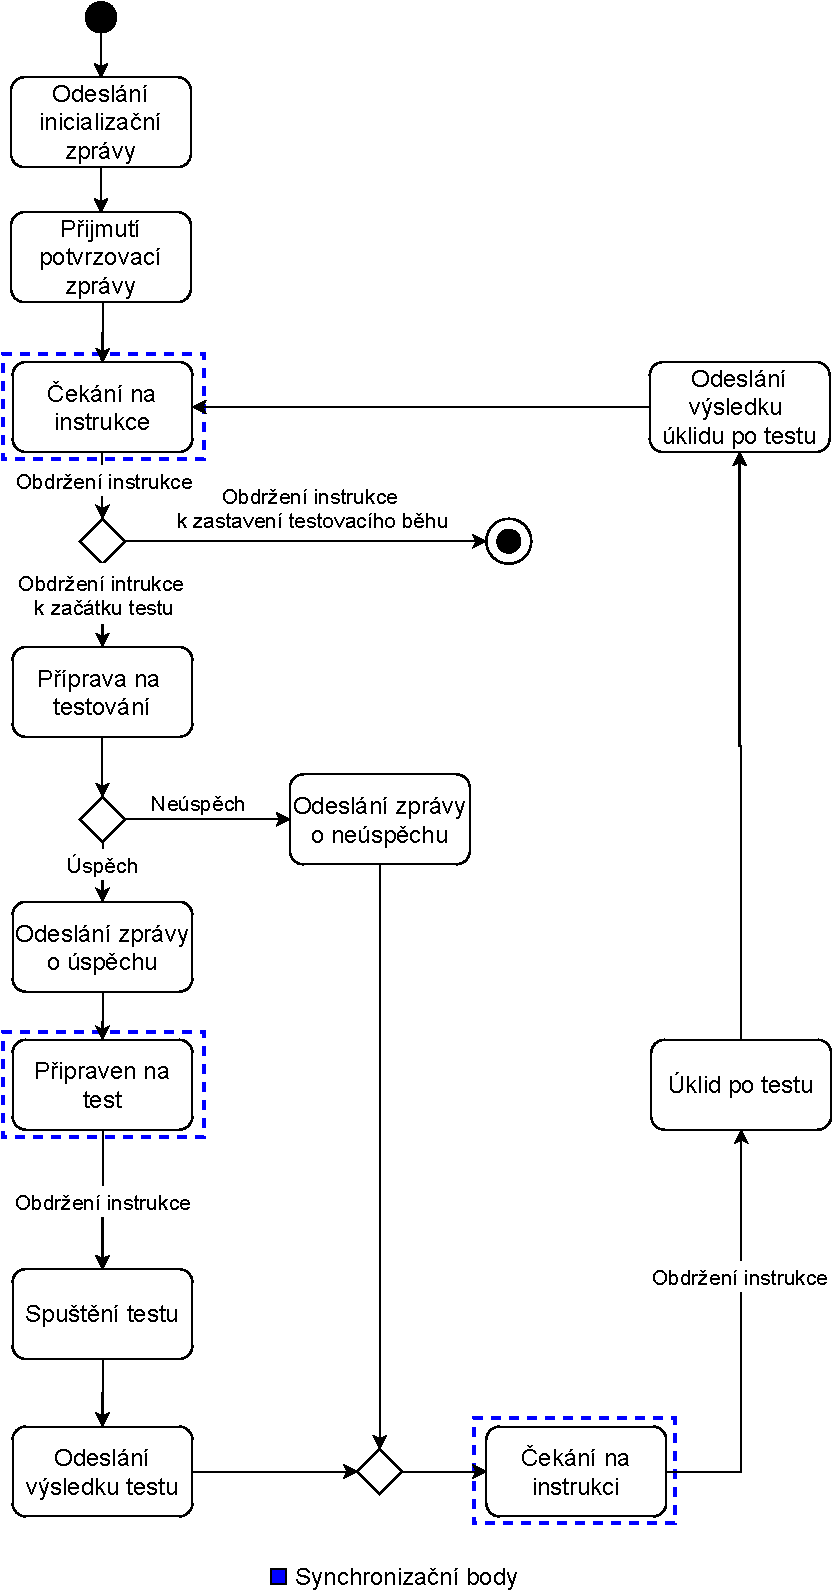
\includegraphics[height=0.98\textheight]{assets/img/bp_assets/activitydiagramdevice.pdf}
    \caption{Diagram aktivit účastníka testu}
    \label{fig:act_diag_device}
\end{figure}



